\chapter[Targeted Optimisation of Atomic Networks]{Targeted Optimisation of \\ Atomic Networks}
\label{ch:targetedopt}

\begin{chapterabstract}
A targeted optimisation method is presented which enables \td{} networks to be constructed by reference to a set of ring statistics and the \aw{} parameter, $\alpha$, which controls the preferred nearest\--neighbour spatial correlations.
The method efficiently utilises the dual lattice and allows systematic exploration of configurational space. 
Three different systems are considered; a system containing 5\--, 6\-- and 7\--membered rings only (a proxy for amorphous graphene), the configuration proposed by Zachariasen, and those
observed experimentally for ultra\--thin films of \sioii. 
The system energies are investigated as a function of the network topologies and the range of physically\--realisable structures established and compared to known experimental results.
The limits on the parameter $\alpha$ are discussed and compared to previous results, whilst the evolution of the network structure as a function of topology is discussed in terms of the ring\--ring pair distribution functions.
\end{chapterabstract}


\section{Disorder in Two\--Dimensional Networks}

As mentioned in previous sections \davidnote{link}, the characterisation of the disorder in \td{} networks can be achieved through the ring structure. 
For three\--coordinate atomic materials the mean ring size is constrained to six by Euler's law, which allows the variance of the ring size distribution, $\mu_2$, to act as a proxy measure for disorder (see sections \ref{s:eulerslaw}, \ref{s:lemaitre}).
The same set of ring statistics can however lead to a large number of different ring arrangements, as shown in figure \ref{fig:zach}.
These can be further quantified by the \aw{} parameter, which measures the ring\--ring correlations.
An interesting observation across a wide range of experimental systems, is that the measured value of the \aw{} parameter is in a tight range of $\alpha\approx0.15\rightarrow 0.3$ \cite{Zsoldos1999}.
This is also effect is also seen in computational studies, including for example the previous chapter.

Whilst it is necessary to capture these measures accurately, and almost by definition good computational models capture the underlying essential physics of a system, they do not give insight into \textit{why} such configurations are preferred. 
To answer this question a different approach is required, where configurations can be systematically generated, covering a parameter space which exceeds the experimentally accessible region.
To achieve this a targeted optimisation method can be employed, whereby configurations are produced to fit network properties, and not driven by an underlying potential model.
This allows the experimentally occurring structures to be viewed in the context of the wider configurational landscape.

\section{Targeted Optimisation Algorithm}

The primary remit of the targeted optimisation algorithm is to generate plausible network configurations based on the supplied network properties of ring statistics and \aw{} parameter.
A secondary requirement is for the method to be efficient enough to produce samples for further high\--throughput calculations.
Both these goals can be successfully accomplished with the method presented here: a \mc{} search algorithm, using the machinery of bond switching.

The bond switching algorithm (described in detail in section \ref{s:bondswitch}), amorphises a crystalline hexagonal lattice by exchanging the neighbouring interactions between pairs of bonded atoms and geometry optimising the structure.
Moves are accepted according to the resulting change in the potential energy, where those with lower energy are accepted with increasing probability.
The driving force is therefore always towards a structure which is physically motivated.
In targeted optimisation, the same Monte Carlo moves are proposed as in bond switching, but crucially moves are not accepted on the basis of the energy of the network, but rather its agreement with a target ring distribution and \aw{} parameter.
This agreement is measured by a cost function of the form:
\begin{equation}
	\label{eq:costfunc}
	\obj=k_\alpha\abs{\alpha-\alpha^t}+\frac{\abs{\mu_2-\mu_2^t}}{\mu_2^t}+\sumk\frac{\abs{p_k-p_k^t}}{p_k^t}\,,
\end{equation} 
where $k_\alpha$ is a scaling constant; $p_k^t$, $\mu_2^t$ and $\alpha^t$ are the input target values; $p_k$ are the system ring statistics; and $\mu_2$ and $\alpha$ are calculated from an \aw{} fit on the current state.
In the cost function the relative difference is used for the ring distribution, as the same accuracy is required for all $p_k^t$, which may differ by several orders of magnitude. 
This is not a concern for $\alpha^t$, which must also have the flexibility to take a zero value, and hence the absolute difference is used in the first term. 

Moves in targeted optimisation are accepted with probability given by the Metropolis condition:
\begin{equation}
	P_{ij}=\min\left[1,\exp{-\Delta\obj/T}\right]\,,
\end{equation}
where $\Delta\obj$ is the difference in cost functions before and after the proposed move, and $T$ is a temperature parameter. 
In contrast to bond switching which is concerned with sampling, this is a global optimisation algorithm and moves are proposed until the network has converged to the target properties and the cost function is zero.
As is the case with such optimisation techniques, steps must be taken to avoid becoming trapped in local minima, and the calculation not converging. 
This is achieved through selection of the parameters $k_\alpha$ and $T$. 
The parameter $k_\alpha$ changes the relative costs of satisfying the $\alpha^t$ and $p_k^t$ conditions, and must be chosen so that neither is overweighted. The parameter $T$ controls the proportion of moves which are accepted. 
Some temperature is required to overcome local minima, but if set too high the algorithm will no longer move downhill in cost and the search becomes effectively random \-- invariably leading to non\--convergence. 
Values for $k_\alpha$ and $T$ can be determined from a parameter search checking for convergence of target systems; but $k_\alpha=10$ and $T\sim 10^{-4}$ were appropriate for systems of the type and size described in this work. 

One key point which arises from using a cost function in this way is that there becomes no requirement for accurate on\--the\--fly geometry optimisation of the atomic positions (as there is no need to calculate potential energies).
It is the underlying topology of the network which determines the system properties, which is invariant to the geometry.
The final energy of the system may well be of interest, but this can be evaluated just once at the end of the calculation.
This opens the door for significant speed\--ups through efficient use of the dual lattice.

\subsection{Dual Space Implementation}

Whilst the targeted optimisation algorithm can be employed using atomic positions, there are significant advantages to a dual space implementation.
As discussed in section \ref{s:atomringnetworks}, the ring structure is better described through the use of the dual network. 
In this representation the ring statistics in equation \eqref{eq:costfunc} are simply given by the node degree distribution. 
In addition, the mean ring sizes about each ring, $m_j$, required for the Aboav\--Weaire fit (equation \eqref{eq:aboavweaire}) can be easily calculated from the joint degree distribution:
\begin{equation}
	m_j = \sumk \frac{ke_{jk}}{q_k}\,.
\end{equation}
Hence, by utilising the ring network, the book\--keeping to track the network properties becomes trivial.

\begin{figure}[bt]
     \centering
     
     \begin{subfigure}[b]{0.3\textwidth}
         \centering
         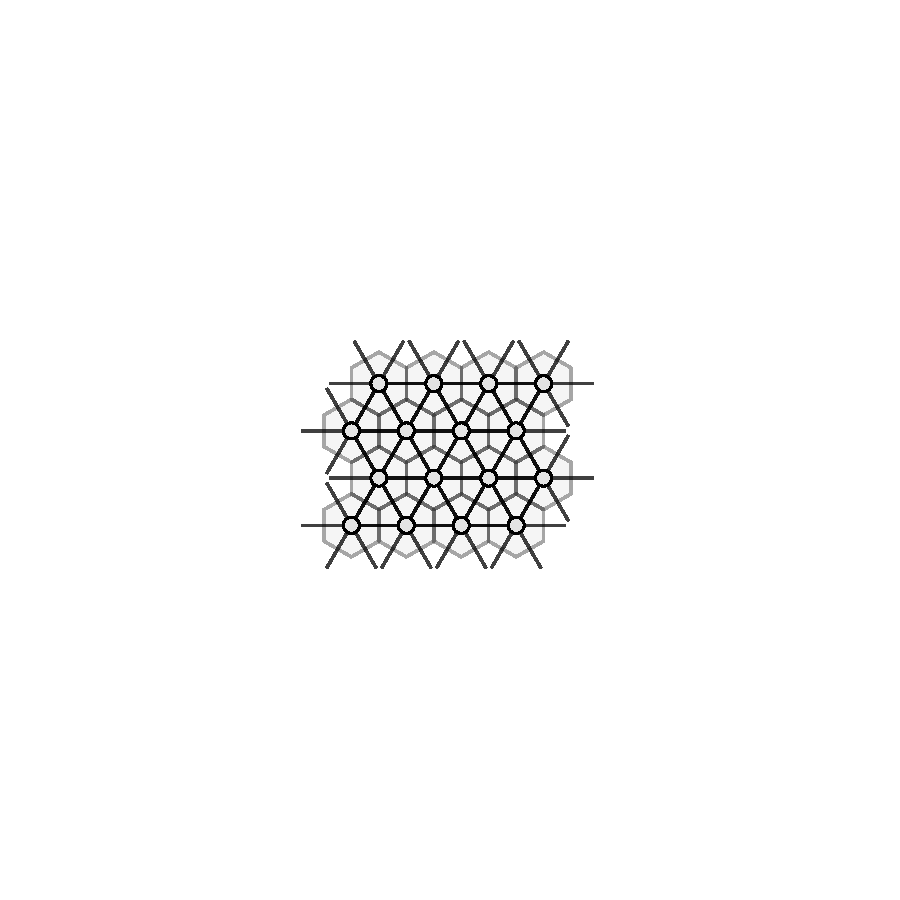
\includegraphics[height=3cm]{./figures/targeted_opt/dualswitch_0.pdf}
         \vspace{-1mm}
         \caption{}
         \label{fig:dualswitch1}
     \end{subfigure}
     \hfill
	\begin{subfigure}[b]{0.3\textwidth}
         \centering
         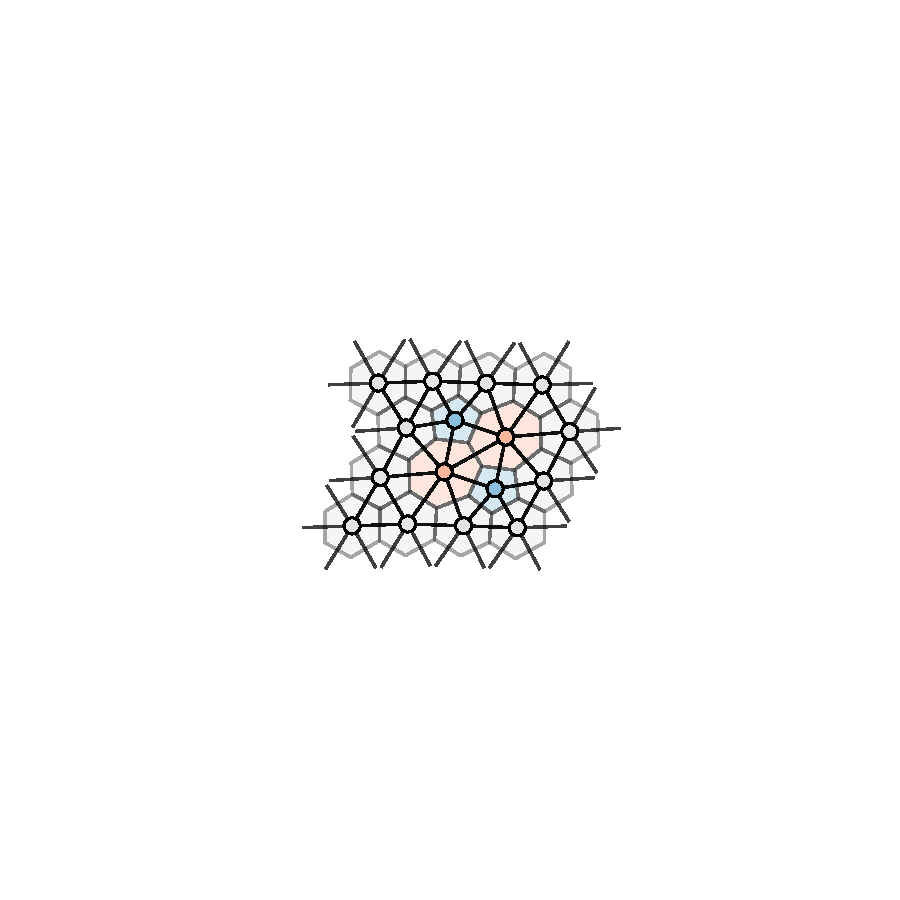
\includegraphics[height=3cm]{./figures/targeted_opt/dualswitch_1.pdf}
         \caption{}
         \label{fig:dualswitch2}
     \end{subfigure}
     \hfill
     \begin{subfigure}[b]{0.3\textwidth}
         \centering
         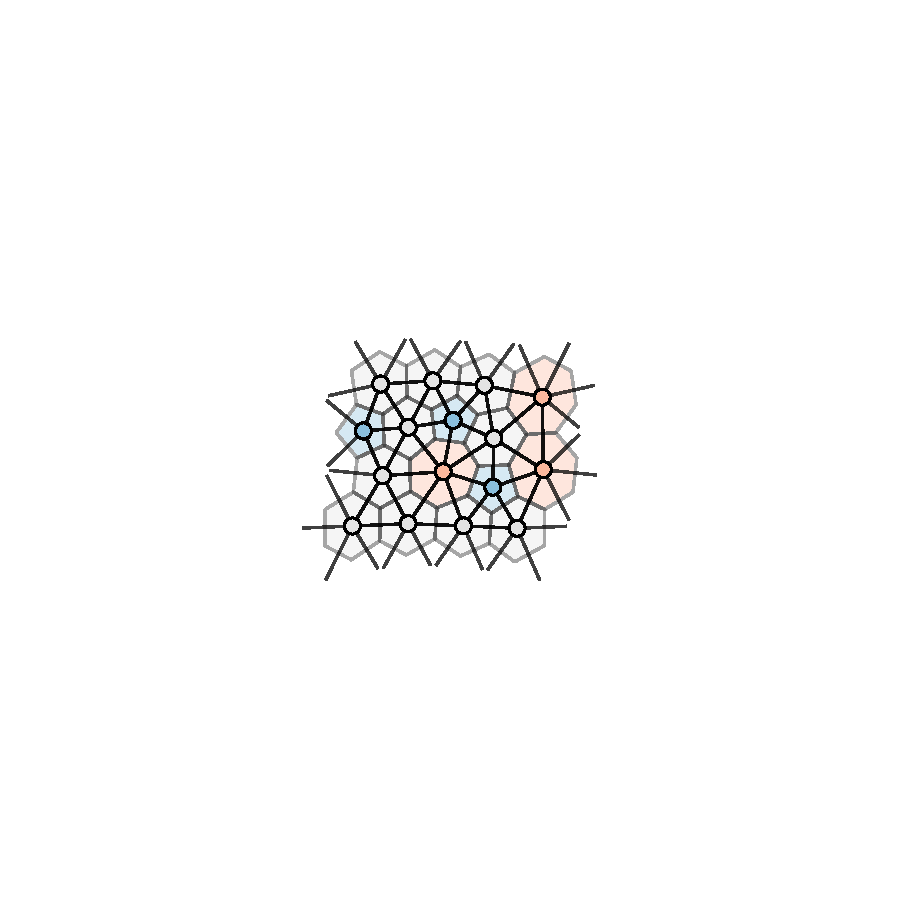
\includegraphics[height=3cm]{./figures/targeted_opt/dualswitch_2.pdf}
         \caption{}
         \label{fig:dualswitch3}
     \end{subfigure}

     \caption{Bond switching \mc{} moves can be performed solely through the dual lattice. Two successive moves are shown from (a)\--(b) and (b)\--(c). In the dual lattice (bold circles and lines) two edge\--sharing triangles are selected and the shared edge transposed. The atomic network is also shown (faded rings) to illustrate the corresponding effect on the atomic structure.}
     \label{fig:dualswitch}
\end{figure}

The implementation of the bond switching move itself is also straightforward in dual space.
Figure \ref{fig:dualswitch} shows how an atomic system can be manipulated \textit{solely} through the dual lattice.
Here the triangular nature of the dual (reflecting the trivalency of the atoms) can be exploited to good effect.
By selecting edge sharing triangles in the ring network and transposing the shared edge connection, a perturbation equivalent to the Stone\--Wales defect can be enacted. 
This process can be continued to generate an amorphous network. 
In addition, although there is no requirement for geometry optimisation after each step, the triangle lattice can be used to cheaply maintain a semi\--phyical structure.
By applying a harmonic potential between all pairs of linked nodes \davidnote{link} etc etc etc. physical, regenerate atomic positions, speedy








